\documentclass[11pt, uplatex, dvipdfmx]{jsarticle}
\usepackage{amsmath,amsfonts, bm, braket, setspace, emathEy, enumerate, graphicx}

\newcommand*{\ds}{\displaystyle}
\renewcommand*{\dlim}{\lim\limits} %emathEyを使わないなら\newcommand
\renewcommand*{\vec}[1]{\overrightarrow{\textrm{#1}}}

\resettagform


\pagestyle{plain}



\title{\Huge 線形代数 問題集}


\begin{document}

\maketitle
\thispagestyle{empty}

\newpage

\section{行列の演算}\label{sec:matrix}

\begin{enumerate}[\ref{sec:matrix}.1]
  \setlength{\itemsep}{1zh}
  
\item 次の行列 $A$ に対し,$A^n$ を求めよう.ただし,$n$ は自然数とする.

  \vspace{1ex}
  
  \begin{edaenumerate}<retusuu=3>[(1)]
  \item $A= \left[
      \begin{array}{rr}
        2 & 1\\
        0 & 2
      \end{array}
    \right]$

  \item $A=\left[
      \begin{array}{rrr}
        2 & 1 & 0\\
        0 & 2 & 0\\
        0 & 0 & 3
      \end{array}
    \right]$
    
  \item $A=\left[
      \begin{array}{rrr}
        2 & 1 & 0\\
        0 & 2 & 1\\
        0 & 0 & 2
      \end{array}
    \right]$
  \end{edaenumerate}\vspace{-2zh}

\item $B=\left[
    \begin{array}{rr}
      2 & 1\\
      0 & 2
    \end{array}
  \right], \; P=\left[
    \begin{array}{rr}
      3 & 4\\
      2 & 3
    \end{array}
  \right]$ とする.

  \vspace{1zh}
  
  \begin{enumerate}[(1)]
    \setlength{\itemsep}{1ex}
    
  \item $P^{-1}AP=B$ となる行列 $A$ を求めよう.

  \item 自然数 $n$ に対し,$A^n$ を求めよう.
  \end{enumerate}

\item $A=\left[
    \begin{array}{rr}
      -2 & 2\\
      5 & -3
    \end{array}
  \right]$ とする.

  \vspace{1zh}

  \begin{enumerate}[(1)]
    \setlength{\itemsep}{1ex}
    
  \item $A^2+5A-4E_2$ を計算しよう.

  \item (1) の結果を活用して $A^5$ を効率良く計算しよう.
  \end{enumerate}
  
\item 下図のような $5$ 個の空港 $1, 2, 3, 4 ,5$ を結ぶ航空路線がある.
  空港 $i$ から空港 $j$ への直通路線があるとき $a_{ij}=1$ とし,そうで
  ないとき $a_{ij}=0$ とする.ただし,$a_{ii}=0$ とする.
  \begin{figure}[h]
    \centering
    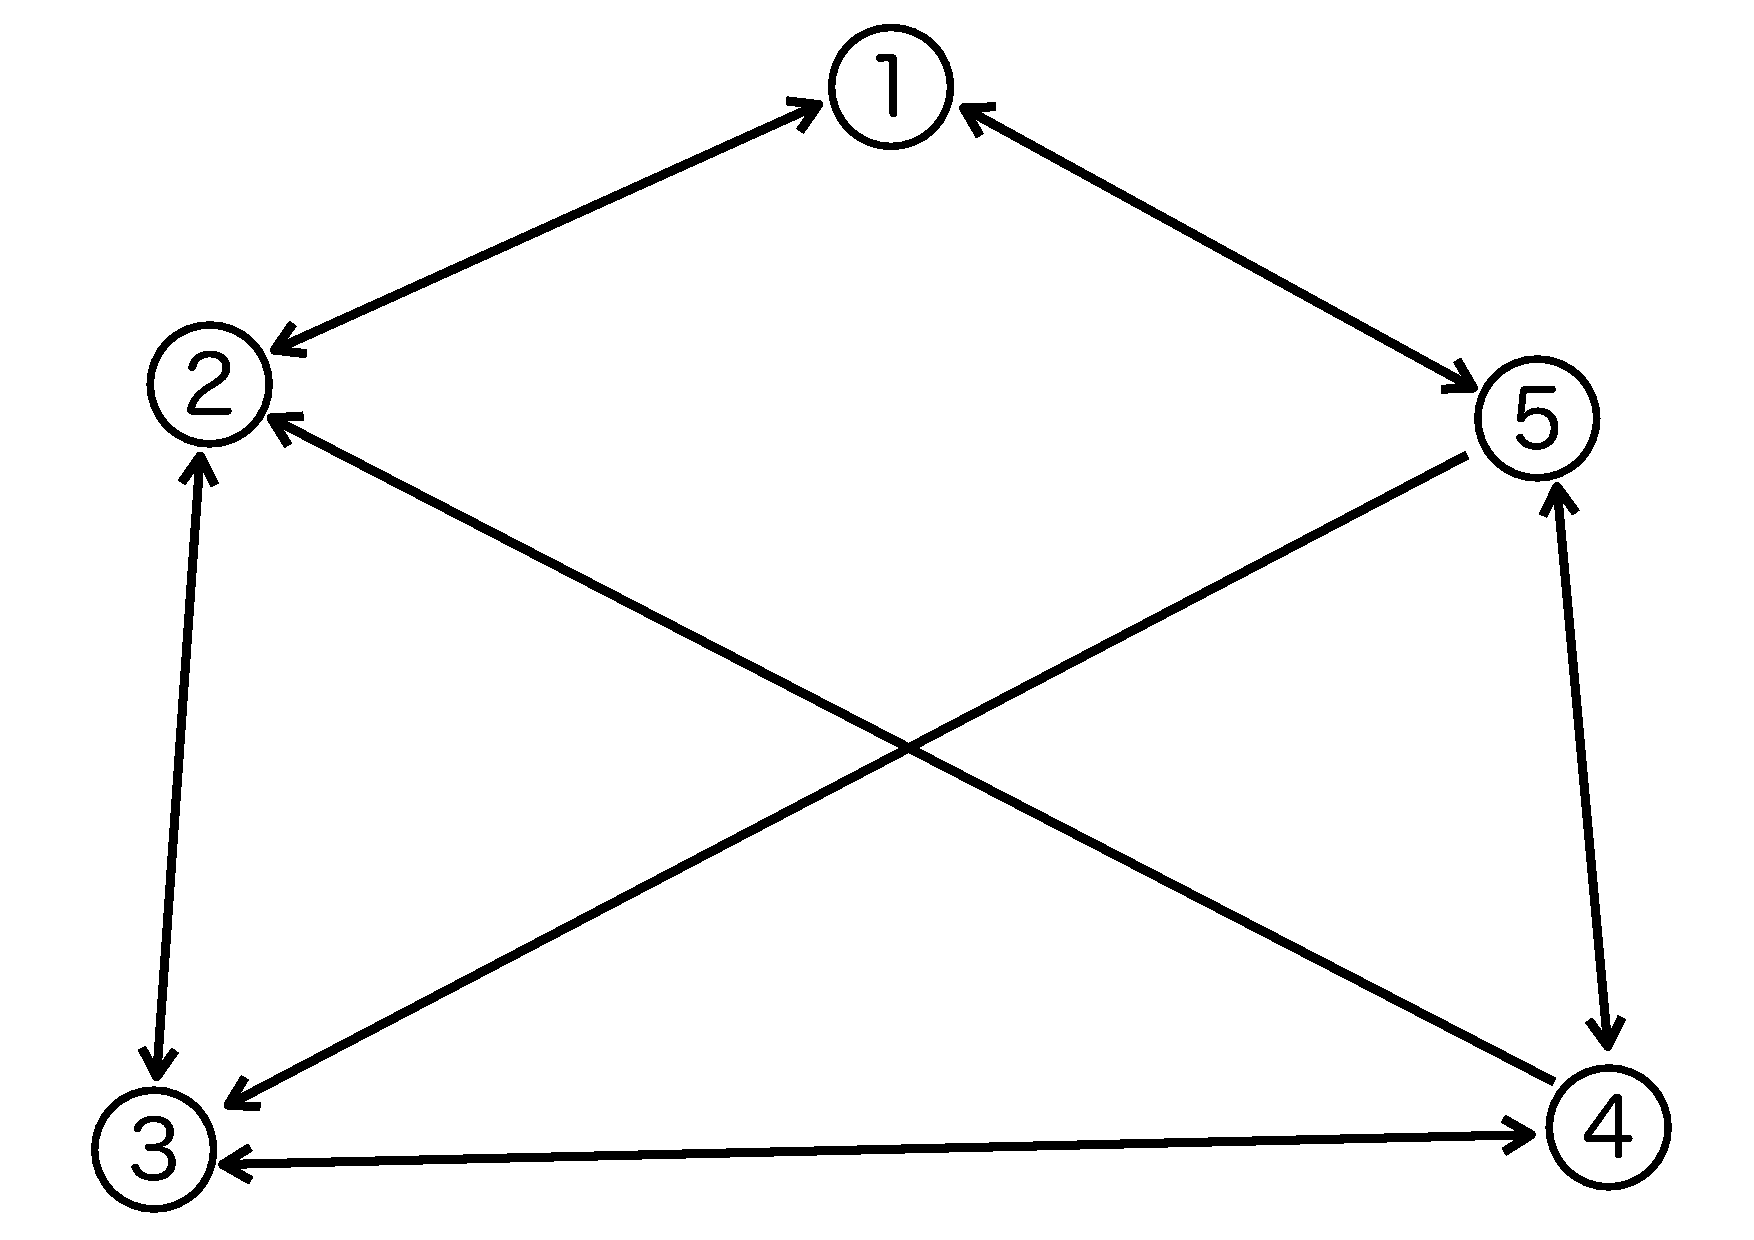
\includegraphics[width=6cm]{./pictures/routes.pdf}
  \end{figure}

  \begin{enumerate}[(1)]
    \setlength{\itemsep}{1ex}
    
  \item $a_{ij}$ を $(i,j)$ 成分とする $5$ 次正方行列 $A=\left[ a_{ij}\right]$ を具体的に書いてみよう.

  \item $A^2, A^3, A^4$ を計算しよう.

  \item $A^2$ の $(i,j)$ 成分は
    $a_{i1} a_{1j} + a_{i2}a_{2j} + a_{i3}a_{3j} + a_{i4}a_{4j} +
    a_{i5}a_{5j}$ であることから,この値が何を意味するか考えよう.

  \item 自然数 $n$ に対して $A^n$ の $(i,j)$ 成分が何を意味するか考えよう.

  \item 路線 $4 \to 2 \to 1 \to 5 \to 3$ のように,空港 $4$ から出発し
    て $4$ 回の移動($3$ 回の乗り継ぎ)で空港 $3$ に到着する路線の個数
    を求めよう.
  \end{enumerate}


\end{enumerate}

\section{行列の基本変形}\label{sec:transform}

以下の \ref{sec:transform}.\ref{trans:mul},
\ref{sec:transform}.\ref{trans:switch},
\ref{sec:transform}.\ref{trans:add}で定義する行列
$M_n(i;c), S_n(i,j), A_n(i,j;c)$ を(行の)基本行列という.


\begin{enumerate}[\ref{sec:transform}.1]
  \setlength{\itemsep}{1zh}
  
\item \label{trans:mul}$n$ 次単位行列 $E_n$ の $(i,i)$ 成分を $c$ で置き換えた行列を $M_n(i ; c)$ とする.

  \vspace{1ex}

  \begin{enumerate}[(1)]
    \setlength{\itemsep}{1ex}
    
  \item $M_3(1; 3), \; M_3(2; -2)$ を具体的に書いてみよう.

  \item $3$ 次正方行列 $A=\left[ a_{ij}\right]$ に対し,行列の
    積 $M_3(1;3)A$ と $M_3(2; -2) A$ を計算しよう.

  \item $M_n(i;c)$ を左から掛けることは何を意味するかを考えよ
    う.
  \end{enumerate}

\item \label{trans:switch}$n$ 次単位行列 $E_n$ の $(i,i)$ 成分と $(j,j)$ 成分を $0$ に,$(i,j)$ 成分
  と $(j,i)$ 成分を $1$ に置き換えた行列を $S_n(i,j) \; (i \neq j)$ とする.

  
  \vspace{1ex}

  \begin{enumerate}[(1)]
    \setlength{\itemsep}{1ex}
    
  \item $S_3(1,2), \; S_3(2, 3)$ を具体的に書いてみよう.

  \item $3$ 次正方行列 $A=\left[ a_{ij}\right]$ に対し,行列の
    積 $S_3(1,2)A$ と $S_3(2,3)A$ を計算しよう.

  \item $S_n(i,j)$ を左から掛けることは何を意味するかを考えよう.
  \end{enumerate}

\item \label{trans:add}$n$ 次単位行列 $E_n$ の $(i,j)$ 成分を $c$ で置き換えた行列
  を $A_n(i,j;c) \; (i \neq j)$ とする.

  \vspace{1ex}

  \begin{enumerate}[(1)]
    \setlength{\itemsep}{1ex}
    
  \item $A_3(1,2 ; 3), \; A_3(3, 2; -1)$ を具体的に書いてみよう.

  \item $3$ 次正方行列 $A=\left[ a_{ij}\right]$ に対し,行列の積 $A_3(1,2; 3)A$ と $A_3(3,2; -1)A$ を計算しよう.

  \item $A_n(i,j; c)$ を左から掛けることは何を意味するかを考えよう.
  \end{enumerate}

\item $A=\left[
    \begin{array}{rrr}
      0 & 3 & 6\\
      1 & 4 & 7\\
      2 & 5 & 8
    \end{array}
  \right]$ とし,$B=\left[ A \  \ E_3\right] = \left[
    \begin{array}{rrrrrr}
      0 & 3 & 6 & 1 & 0 & 0\\
      1 & 4 & 7 & 0 & 1 & 0\\
      2 & 5 & 8 & 0 & 0 & 1
    \end{array}
  \right]$ とする.

  \vspace{1zh}

  \begin{enumerate}[(1)]
    \setlength{\itemsep}{1ex}
    
  \item 行列の積 $S_3(1,2) B$ と $A_3(3,1; -2) S_3(1,2)B$ を計算しよう.

  \item $A$ の簡約化を $C$ とする.$PA=C$ となる $3$ 次正方行列 $P$ を求めよう.
    
  \end{enumerate}
  
\item $\bm{a}_1=\left[
    \begin{array}{r}
      1\\
      1\\
      2
    \end{array}
  \right], \; \bm{a}_2=\left[
    \begin{array}{r}
      1\\
      0\\
      1
    \end{array}
  \right], \; \bm{a}_3=\left[
    \begin{array}{r}
      2\\
      2\\
      1
    \end{array}
  \right], \quad A=\left[
    \begin{array}{ccc}
      \bm{a}_1 & \bm{a}_2 & \bm{a}_3
    \end{array}
  \right]$ とする.

  \vspace{1zh}

  \begin{enumerate}[(1)]
    \setlength{\itemsep}{1ex}

  \item 行列の積 ${}^{t}A A$ を計算しよう.
    
  \item 内積 $\bm{a}_i \cdot \bm{a}_j$ を $(i,j)$ 成分とする $3$ 次正方
    行列 $G=\left[ \bm{a}_i \cdot \bm{a}_j\right]$ を計算しよう.

  \item $L=A_3(3,1,-1) A_3\left(2,1,-\frac{1}{2}\right)$ とす
    る.行列の積 $LG$ と $L ({}^{t}A)$ を計算しよう.

  \item $B={}^{t}\left( L ({}^{t}A)\right)$ とする.行列の積 ${}^{t} B  B$ を計算しよう.
    
    
  \end{enumerate}
\end{enumerate}

\newpage

\section{連立1次方程式}\label{sec:system}

\begin{enumerate}[\ref{sec:system}.1]

  \setlength{\itemsep}{1zh}


\item 次の行列 $A, B$ に対して,$AX=B$ を満たす行列 $X$ を全て求めよう.

  \vspace{1ex}
  
  \begin{enumerate}[(1)]
    \setlength{\itemsep}{1zh}
    
  \item $A= \left[
      \begin{array}{rr}
        1 & 2\\
        3 & 4
      \end{array}
    \right] , \quad B=\left[
      \begin{array}{rr}
        9 & 5\\
        21 & 9
      \end{array}
    \right]$

  \item $A=\left[
      \begin{array}{ccc}
        1 & 2 & 3\\
        4 & 5 & 6\\
        7 & 8 & 9
      \end{array}
    \right], \quad B=\left[
      \begin{array}{rrr}
        -3 & 6 & 4\\
        3 & 9 & 16\\
        9 & 12 & 28
      \end{array}
    \right]$
  \end{enumerate}

\item 以下を満たす $3$ 次関
  数 $f(x)=a_0 + a_1 x + a_2 x^2 + a_3 x^3$ の係数を決定しよう.
  \[
    f(1)=1, \quad f(2)=2, \quad f'(1)=2, \quad f'(2)=3
  \]
  
\item $xy$ 平面において $a x^2 + bxy + cy^2 + dx + ey + f=0$ という形
  の $2$ 次方程式によって定まる曲線を $2$ 次曲線という.以下
  の $5$ 点 A, B, C, D, E を通る $2$ 次曲線の方程式を求めよう.
  \[
    \textrm{A}(3,-1), \quad \textrm{B}(2,2), \quad \textrm{C}(-4,-1),
    \quad \textrm{D}(-1,-2), \quad \textrm{E}(0,-4)
  \]

\item 4つの物質 A, B, C, D を含む混合溶液 W, X, Y, Z がある.これら4つ
  の混合溶液を適切な割合で混ぜ合わせて新たな溶液 $\Omega$ を作りたい.
  以下の表は各溶液 W, X, Y, Z とこれから作りたい溶液 $\Omega$ の100gあ
  たりに含まれる物質 A, B, C, D の含有量(単位はg)を表したものである.
  各溶液を混ぜ合わせることで化学反応等による質量欠損は起きないものとし
  て,混ぜ合わせる溶液 W, X, Y, Z の適切な割合を求めよう.
\begin{table}[h]
  \centering
  \begin{tabular}{ccccc|c}
    & W & X & Y & Z & $\Omega$\\ \hline
    A & 2.00 & 1.00 & 4.00 & 9.00 & 3.00\\ \hline
    B & 7.00 & 10.0 & 1.00 & 2.00 & 6.00\\ \hline  
    C & 2.00 & 2.00 & 2.00 & 2.00 & 2.00 \\ \hline
    D & 4.00 & 8.00 & 10.0 & 7.00 & 7.00\\ 
  \end{tabular}
\end{table}

  
\item $\bm{a}_1 = \left[
    \begin{array}{r}
      2\\
      2\\
      -1
    \end{array}
  \right], \; \bm{a}_2=\left[
    \begin{array}{r}
      1\\
      3\\
      -4
    \end{array}
  \right], \; \bm{b} = \left[
    \begin{array}{r}
      5\\
      2\\
      5
    \end{array}
  \right], \; A=\left[
    \begin{array}{cc}
      \bm{a}_1 & \bm{a}_2
    \end{array}
  \right]$ とする.
      
  \vspace{1zh}

  
  \begin{enumerate}[(1)]
    \setlength{\itemsep}{1ex}
    
  \item 連立1次方程式 $A\bm{x} = \bm{b}$ を解こう.

  \item 連立 $1$ 次方程式 ${}^{t}A A\bm{x} = {}^{t}A \bm{b}$ を解こう.

  \item (2) で求めた解 $\bm{x}$ に対して,空間ベクトルの内
    積 $(A\bm{x}) \cdot (A\bm{x} -\bm{b})$ を計算しよう.

  \item 空間ベクトル $A\bm{x}-\bm{b}$ の大きさの $2$ 乗 $|A\bm{x} - \bm{b}|^2$ が最小とな
    る $\bm{x}$ を求めよう.
  \end{enumerate}
    
\end{enumerate}

\newpage

\section{行列式}\label{sec:determinant}

\begin{enumerate}[\ref{sec:determinant}.1]
  \setlength{\itemsep}{1zh}
  
\item 

  \begin{enumerate}[(1)]
    \setlength{\itemsep}{1ex}
    
  \item O を原点とする $xy$ 平面上に $3$ 点 A$(a,c)$, B$(b,d)$,
    C$(a+b, c+d)$ があり,$\vec{OA}$ と $\vec{OB}$ は平行でないとする.
    平行四辺形 OACB と三角形 OAB の面積を求めよう.

  \item $2$ 次正方行列 $\left[
      \begin{array}{cc}
        a & b\\
        c & d
      \end{array}
    \right]$ の行列式を計算しよう.

  \item $5$ 点 P$(4,4)$, Q$(-2,6)$, R$(-5,1)$, S$(-3,-3)$, T$(5,-3)$ を
    頂点とする五角形 PQRST の面積を求めよう.
  \end{enumerate}

\item 空間ベクトル $\bm{a} = {}^{t}\left[
    \begin{array}{ccc}
      a_1 & a_2 & a_3
    \end{array}
  \right], \; \bm{b}=  {}^{t}\left[
    \begin{array}{ccc}
      b_1 & b_2 & b_3
    \end{array}
  \right]$ に対して
  \[
    \bm{a} \times \bm{b} = \left|
      \begin{array}{cc}
        a_2 & b_2\\
        a_3 & b_3
      \end{array}
    \right| \bm{e}_1 -\left|
      \begin{array}{cc}
        a_1 & b_1\\
        a_3 & b_3
      \end{array}
    \right|\bm{e}_2 + \left|
      \begin{array}{cc}
        a_1 & b_1\\
        a_2 & b_2
      \end{array}
    \right| \bm{e}_3 = \left|
      \begin{array}{ccc}
        a_1 & b_1 & \bm{e}_1\\
        a_2 & b_2 & \bm{e}_2\\
        a_3 & b_3 & \bm{e}_3
      \end{array}
    \right|
  \]
  を $\bm{a}$ と $\bm{b}$ の外積という.($\bm{e}_1, \bm{e}_2,
  \bm{e}_3$ を形式的に数のように扱って行列式を計算する)

  \vspace{1ex}

  \begin{enumerate}[(1)]
    \setlength{\itemsep}{1ex}
    
  \item 内積 $\bm{a} \cdot (\bm{a} \times \bm{b})$ と $\bm{b}\cdot ( \bm{a} \times \bm{b})$ を計算しよう.

  \item 空間ベクトル $\bm{a} \times \bm{b}$ の大きさ $|\bm{a} \times \bm{b}|$ を求めよう.

  \item 空間ベクトル $\bm{a}$ と $\bm{b}$ が張る平行四辺形の面積を求めよう.
    
  \end{enumerate}

\item ${}^{t}\bm{a}=\left[
    \begin{array}{ccc}
      a_1 & a_2 & a_3
    \end{array}
  \right], \; {}^{t}\bm{b}=\left[
    \begin{array}{ccc}
      b_1 & b_2 & b_3
    \end{array}
  \right], \; {}^{t}\bm{c} = \left[
    \begin{array}{ccc}
      c_1 & c_2 & c_3
    \end{array}
  \right]$ とする.

  \vspace{1zh}
  
  \begin{enumerate}[(1)]
    \setlength{\itemsep}{1ex}
    
  \item 空間ベクトル $\bm{a}$ と $\bm{b}$ と $\bm{a} \times \bm{b}$ が
    張る平行六面体の体積を求めよう.
    
  \item 空間ベクトル $\bm{a}$ と $\bm{b}$ と $\bm{c}$ が張る平行六面体の体積を求めよう.

  \item 空間ベクトルの内積 $(\bm{a} \times \bm{b}) \cdot \bm{c}$ を計算しよう.

  \item $3$ 次正方行列 $A=\left[
      \begin{array}{ccc}
        \bm{a} & \bm{b} & \bm{c}
      \end{array}
    \right]$ の行列式を計算しよう.
      
  \end{enumerate}
  
\item $xyz$ 空間の以下の $4$ 点 O, A, B, C を頂点とする四面
  体 OABC の体積と表面積を求めよう.
  \[
    \textrm{O}(0,0,0), \quad \textrm{A}(3,0,-3), \quad \textrm{B}(2,2,4), \quad \textrm{C}(-2,1,1)
  \]


\item $\bm{a}_1=\left[
    \begin{array}{r}
      1\\
      1\\
      2
    \end{array}
  \right], \; \bm{a}_2=\left[
    \begin{array}{r}
      1\\
      0\\
      1
    \end{array}
  \right], \; \bm{a}_3=\left[
    \begin{array}{r}
      2\\
      2\\
      1
    \end{array}
  \right], \; g_{ij} = \bm{a}_i \cdot \bm{a}_j \; (1 \leqq i,j \leqq 3)$ とする.

  \vspace{1zh}

  \begin{enumerate}[(1)]
    \setlength{\itemsep}{1ex}
    
  \item $\bm{b}_1 = \bm{a}_1, \quad \bm{b}_2= \left|
      \begin{array}{cc}
        g_{11} & g_{12}\\
        \bm{a}_1 & \bm{a}_2
      \end{array}
    \right|, \quad \bm{b}_3 = \left|
      \begin{array}{ccc}
        g_{11} & g_{12} & g_{13}\\
        g_{21} & g_{22} & g_{23}\\
        \bm{a}_1 & \bm{a}_2 & \bm{a}_3
      \end{array}
    \right|$ を計算しよう.

  \item $3$ 次正方行列 $B=\left[ \bm{b}_i \cdot \bm{b}_j\right]$ を計算しよう.
  \end{enumerate}
\end{enumerate}

\newpage

\section*{解答}

\begin{enumerate}[\ref{sec:matrix}.1]
  \setlength{\itemsep}{1ex}
  
\item
  \begin{enumerate}[(1)]
    \setlength{\itemsep}{1ex}
    
  \item 
  \end{enumerate}

\item

\item
\end{enumerate}

\end{document}
